Today we'll outline the content of this course and motivate it with a few examples. To begin with, symmetry as a principle has led physicists all the way to our current model of physics. This course's content will be almost exclusively mathematical, yet more pragmatic about introducing the necessary tools to apply symmetries to the physical systems we're interested in.

\subsection*{Resources}
\begin{itemize}
    \item Notes (online)
    \begin{itemize}
        \item \href{http://www.damtp.cam.ac.uk/user/examples/3P2.pdf}{Nick Manton's notes} (concise, more on geometry of Lie groups)
        \item \href{http://www.damtp.cam.ac.uk/user/examples/3P2Lb.pdf}{Hugh Osborn's notes} (comprehensive, don't cover Cartan classification)
        \item \href{http://www.damtp.cam.ac.uk/user/examples/3P2Lc.pdf}{Jan Gutowski's notes} (classification of Lie algebras). There is actually a second set of notes on an earlier version of the course which can be found \href{http://personal.maths.surrey.ac.uk/st/jg0033/Resources/lectnotes(master).pdf}{here}, but I believe the notes referred to in lecture are the first set.
    \end{itemize}
    \item Books: ``Symmetries, Lie Algebras and Representations'', Fuchs \& Schweigert Ch. 1-7.
\end{itemize}

\subsection*{Introduction}
\begin{defn}
We define a \term{symmetry} as a transformation of dynamical variables that leaves the form of physical laws invariant.
\end{defn}
\begin{exm}
A rotation is a transformation, e.g. on $\vec{x}\in \RR^3$ such that $\vec{x}'=M\cdot \vec{x} \in \RR^3$. There are \term{orthogonal} matrices which satisfy $MM^T = 1_3$ and also \term{special} matrices which satisfy $\det M = 1$.
\end{exm}

%\subsection*{Mathematical Formulation}
It's also useful for us to define the notion of a group (likely familiar from an intro course on abstract algebra or mathematical methods).

\begin{defn}
A \term{group} $G$ is a set equipped with a multiplication law (binary operation) obeying
\begin{itemize}
    \item Closure ($\forall g_1, g_2\in G, g_1g_2 \in G$)
    \item Identity ($\exists e\in G \text{s.t.} \forall g\in G, eg = ge = g$)
    \item Existence of inverses ($\forall g \in G, \exists g^{-1} \in G$ s.t. $g^{-1}g=gg^{-1}=e$)
    \item Associativity ($\forall g_1,g_2,g_3\in G, (g_1g_2)g_3)=g_1(g_2g_3)$).
\end{itemize}
\end{defn}
\begin{ex}
 For rotations $G=SO(3)$, the group of 3-dimensional special orthogonal matrices, check that the group axioms apply (SO(3) forms a group).
\end{ex}

We also remark that the set may be finite or infinite\footnote{For example, cyclic groups $\ZZ_n$ (i.e. addition in modular arithmetic) vs. most matrix groups like $GL_n$.}. A group $G$ is called \term{abelian} if the multiplication law is commutative ($\forall g_1,g_2\in G, g_1g_2=g_2g_1$). Otherwise, it is called non-abelian.

We notice that a rotation in $\RR^3$ depends continuously on 3 parameters: $\hat n\in S^2, \theta \in[0,\pi]$ (with $\hat n$ the axis of rotation, $\theta$ the angle of rotation). This leads us to introduce the idea of a Lie group.
\begin{defn}
A \term{Lie group} $G$ is a group which is also a smooth manifold. It's key that the group and manifold structures must be compatible, and so $G$ is (almost) completely determined by the behavior ``near'' $e$, i.e. by infinitesimal transformations in a small neighborhood of the identity element $e$. These correspond to the \term{tangent vectors} to $G$ at $e$.
\end{defn}

The tangent vectors are local objects which span the tangent space to the manifold at some given point. It turns out that $\forall v_1,v_2\in T_e(G)$ the tangent space of $G$, we can define a binary operation $[,]:T_e(G)\times T_e(G) \to T_e(G)$ such that $[,]$ is bilinear, antisymmetric, and obeys the Jacobi identity. 
\begin{defn}
The tangent space at the identity equipped with the Lie bracket defines a \term{Lie algebra} $\mathcal{L}(G).$
\end{defn}

%\subsection*{Cartan classification}
It's a remarkable fact that \emph{all} finite-dimensional semi-simple Lie algebras (over $\CC$) can be classified into four infinite families $A_n, B_n, C_n,D_n$ with $n\in \NN$, plus five \term{exceptional cases} $E_6,E_7,E_8,G_2,F_4$.\footnote{The exceptional groups have not yet come up in physical phenomena, but they seem to have a mysterious connection to the absence of anomalies in string theory.} We call this the \term{Cartan classification.}

\subsection*{Symmetries in physics}
In classical physics, (continuous) symmetries give rise to conserved quantities. This is the conclusion of Noether's theorem.
\begin{exm}
Rotations in $\RR^3$ correspond to conservation of angular momentum, $\vec{L}=(L_1,L_2,L_3)$.
\end{exm}
In quantum mechanics, we have
\begin{itemize}
    \item states: vectors in Hilbert space $\ket{\psi}\in \mathcal{H}$
    \item observables: linear operators $\hat O: \mathcal{H}\to\mathcal{H}$ with (generally) non-commutative multiplication.
\end{itemize}
We recall from previous courses in QM that operators which commute with the Hamiltonian (e.g. $[\hat H, \hat L_i]=0, i= 1,2,3$) give rise to ``quantum conserved quantities.''

In fact, we recall that the angular momentum operators are associated to a Lie bracket: $[\hat L_i, \hat L_j]=i \epsilon_{ijk} \hat L_k$. But this is exactly the $\mathcal{L}(SO(3))$ Lie algebra. 

Our angular momentum operators often act on finite-dimensional vector spaces, e.g. \emph{electron spin}.
$$\ket{\uparrow}\equiv \begin{pmatrix}1\\0\end{pmatrix},\ket{\downarrow}\equiv \begin{pmatrix}0\\1\end{pmatrix}$$
This corresponds to a two-dimensional \term{representation} of $\mathcal{L}(SO(3)$, i.e. a set of $2\times 2$ matrices $\Sigma_i, i=1,2,3$ satisfying the same Lie algebra,
$$[\Sigma_i,\Sigma_J]=i\varepsilon_{ijk}\Sigma_k,$$
which is provided by setting $\Sigma_i=\frac{1}{2}\sigma_i$, our old friends the Pauli matrices.

More generally, we should think of a representation as a map $e$ from a Lie group to some space of transformations on a vector space which preserves the Lie bracket, $e([v_1,v_2])=[e(v_1),e(v_2)]$.

Now suppose we have a rotational symmetry in a quantum system, $$[\hat H, \hat L_i]=0,i=1,2,3.$$ Then the spin states obey $\hat H\ket{\uparrow}=E\ket{\uparrow}, \hat H\ket{\downarrow}= E' \ket{\downarrow}$, with $E=E'$. More generally, degeneracies in the energy spectrum of quantum systems correspond to irreducible representations of symmetries.

\begin{exm}
We have an approximate $SU(3)$ symmetry for the strong force, with
$$G=SU(3)\equiv \{3\times 3 \text{ complex matrices } M \text{ with } M M^\dagger = I_3 \text{ and } \det M = 1.\}$$
The spectrum of mesons and baryons are thus defined by the representation of the Lie algebra $\mathcal{L}(SU(3))$. See also the ``eightfold way,'' due to Murray Gell-Mann, who showed that plotting the various mesons and baryons with respect to certain quantum numbers (isospin and hypercharge) gives rise to a very nice picture corresponding to the 8-dimensional representation of the Lie algebra $\mathcal{L}(SU(3)).$
\end{exm}

\begin{figure}
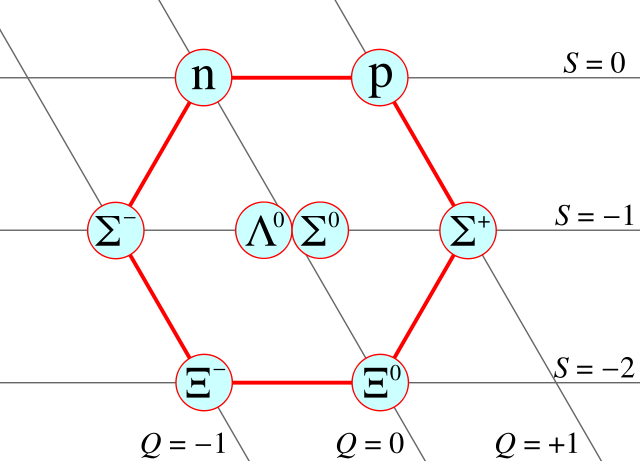
\includegraphics[scale=0.4]{2018/10/20181004_baryonoctet}
\caption{The baryon octet. Particles are arranged by their charge along the diagonals and by their strangeness on the horizontal lines.}
\end{figure}